\subsection{Zielformulierung}

Ziel ist es, eine Anwendung zu schaffen, welche den Anforderungen der Datenverarbeitung innerhalb von Simplex4TwIS gerecht wird. Dabei gibt es zwei Anwendungsbereiche, welche sich in ihren Grundeigenschaften ähneln: das Erstellen von Konvertierungen beim Importieren in das Realitätsmodell (Vgl. \ref{sec:simplex-importer}) und das Erstellen von SimplexSzenarios (Vgl. \ref{sec:simplex-scenarios}).

Das Erstellen von Konvertierungen findet nach dem Einlesen von Ausgangsdaten in die Datenbank statt (Vgl. \ref{sec:simplex-importer}). Dabei entstehen sogenannte Importtabellen, in denen die Informationen in flachen Strukturen enthalten sind. Die Konvertierungen nutzen die Importtabellen dann, um die Daten in das Realitätsmodell zu übertragen.

Sobald sich die Daten im Realitätsmodell befinden, besteht die Möglichkeit, SimplexSzenarios zu definieren. Diese selektieren und kombinieren Attribute aus Objektklassen, um fachspezifische Auswertungen zu generieren. Die Erstellung der SimplexSzenarios kann in zwei Schritten erfolgen, wobei im Ersten die gewünschten Objektklassen ausgewählt werden, und im Zweiten die Attribute ausgewählt und miteinander kombiniert werden. Diese Arbeit beschränkt sich dabei auf den zweiten Schritt.

Beide Prozesse erfordern manuelle Angaben, die bestimmen wie aus den Ausgangsdaten (Importtabellen oder Objektklassen) Zielstrukturen (Objekte oder SimplexSzenarios) erstellt werden sollen. In beiden Fällen ist das Format der Ausgangsdaten klar definiert, da Attribut-Schlüssel und Datentypen gegeben sind. Im Falle der Konvertierungen ist auch das Zielformat festgelegt, da das Schema der Objektklasse (Standardfelder und Sachattribute) bereits definiert wurde. Bei SimplexSzenarios ist dies nicht der Fall, denn die darin enthaltenen Attribute können während der Erstellung frei angelegt werden. Sowohl in Konvertierungen als auch in SimplexSzenarios ist es möglich, Funktionen auf Attribute, beziehungsweise Datenbankspalten anzuwenden. Dabei handelt es sich um Standard-\ac{SQL}-Funktionen oder solche, die durch Erweiterungen\footnote{wie beispielweise PostGIS, eine PostgreSQL-Erweiterung für Geodaten \parencite{postgispscPostGIS}} zur Verfügung gestellt werden. Außerdem können im Zuge beider Arbeitsschritte Filterbedingungen definiert werden, um nur bestimmte Zeilen der Importtabelle in Objekte umzuwandeln oder um nur bestimmte Objekte in SimplexSzenarios auszuwerten.

Aufgrund der genannten Gemeinsamkeiten soll ein Editor entwickelt werden, welcher sowohl für die Erstellung von Konvertierungen als auch für die Definition von SimplexSzenarios verwendet werden kann. Im zweiten Anwendungsfall unterscheidet sich die Funktionalität dahingehend, dass die Ausgabefelder frei bestimmt und benannt werden können.

Der aktuelle Editor für Konvertierungen besteht aus Textfeldern, in denen Auszüge von \ac{SQL}-Befehlen eingegeben werden können. Ein Beispiel dafür ist in Abbildung \ref{fig:conversion-gemeinde} gegeben. Die eingegebenen Ausdrücke werden dann in einen \texttt{SELECT}-Befehl eingesetzt. Diese Herangehensweise ist äußerst flexibel, weist jedoch in der Benutzung einige Usability-Probleme auf. Eine wesentliche Rolle spielt, dass die Ausgangsdaten nicht innerhalb des Editors dokumentiert sind. Die Benutzer:innen müssen somit immer nachschlagen, welche Werte sie eintragen können. Das manuelle Eintippen birgt außerdem die Gefahr, sowohl Tippfehler als auch Fehler im \ac{SQL}-Syntax zu verursachen. Auch die inhaltliche Sinnhaftigkeit der Befehle wird nicht sichergestellt, und Nutzer:innen, die nicht mit SQL vertraut sind, benötigen aufwendige Einführungen und können komplexe Aufgaben schlechter bewältigen. Im einfachsten Fall muss für das Beispiel (Abbildung \ref{fig:conversion-gemeinde}) die Struktur der Importtabelle bekannt sein, um den Spaltenname \texttt{q.gemeindename} anzugeben. In komplexeren Fällen müssen zudem die Funktion \texttt{LPAD}, der Textverkettungs-Operator \texttt{||}, \texttt{CASE}-Ausdrücke und allgemeiner \ac{SQL}-Syntax bekannt sein, sowie fehlerfrei angewendet werden.

\begin{figure}[ht]
  \centering
  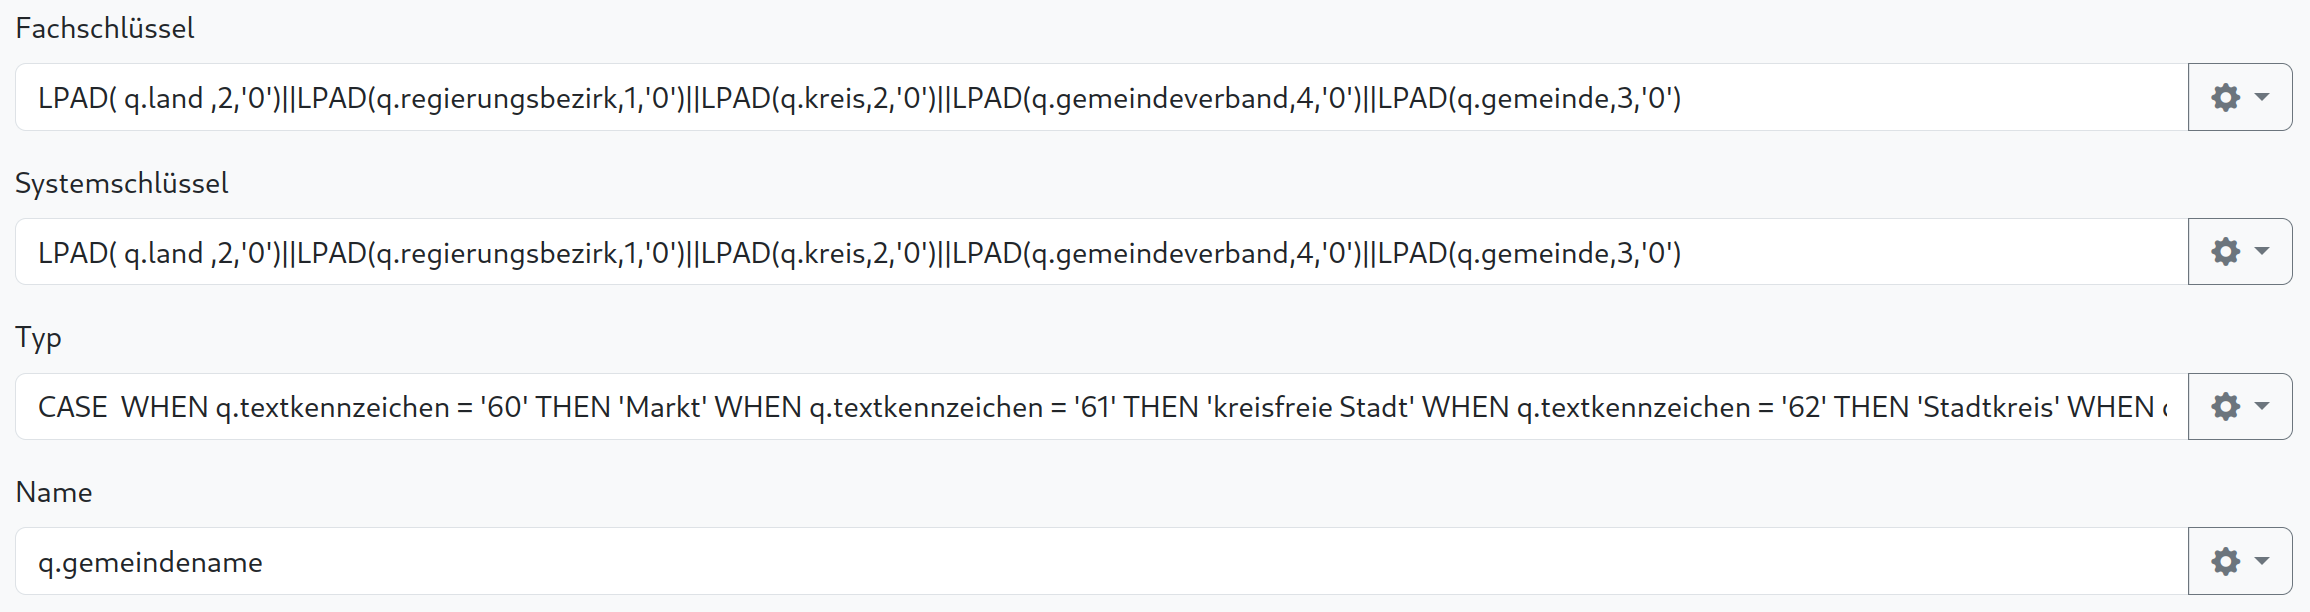
\includegraphics[width=.95\textwidth]{assets/conversion-gemeinde.png}
  \caption[Auszug einer Konvertierungsdefinition im aktuellen Editor]{Auszug aus der Konvertierungsdefinition für die Objektklasse "Gemeinde" im aktuellen Editor für Konvertierungen. Im einfachsten Fall wird der Name der Importtabellenspalte angegeben (siehe Standardfeld "Name"). Der Fach- und Systemschlüssel muss jedoch mit einem Textverkettungsbefehl aus Einzelteilen zusammengesetzt werden. Im Falle des Standardfelds "Typ" wird ein \texttt{CASE}-Befehl genutzt, um Werte aus einer Codeliste zu dekodieren.}
  \label{fig:conversion-gemeinde}
\end{figure}

\pskip
Der entwickelte Editor sollte bezüglich seiner Nutzbarkeit eine Verbesserung gegenüber der aktuellen Lösung darstellen. Zusammenfassend können folgende Ziele formuliert werden:
\begin{itemize}
  \item Entwicklung eines Editors für Konvertierungen und SimplexSzenarios.
  \item Der Editor soll häufiges Nachschlagen verhindern.
  \item Der Editor soll Tippfehler vermeiden.
  \item Der Editor soll auch ohne \ac{SQL}-Kenntnisse bedienbar sein.
\end{itemize}
